\documentclass[legalpaper]{article}
\usepackage[utf8]{inputenc}
\usepackage[spanish]{babel}
\usepackage{graphicx}
\usepackage{float}
\usepackage{subfigure}

\title{Primer documento en \LaTeX}
\author{Brian Bautista}

\begin{document}
    \maketitle
    Hola mundo desde \LaTeX, soy Brian y quiero hacer mi primer documento.

    \section*{1. Im\'agenes}

        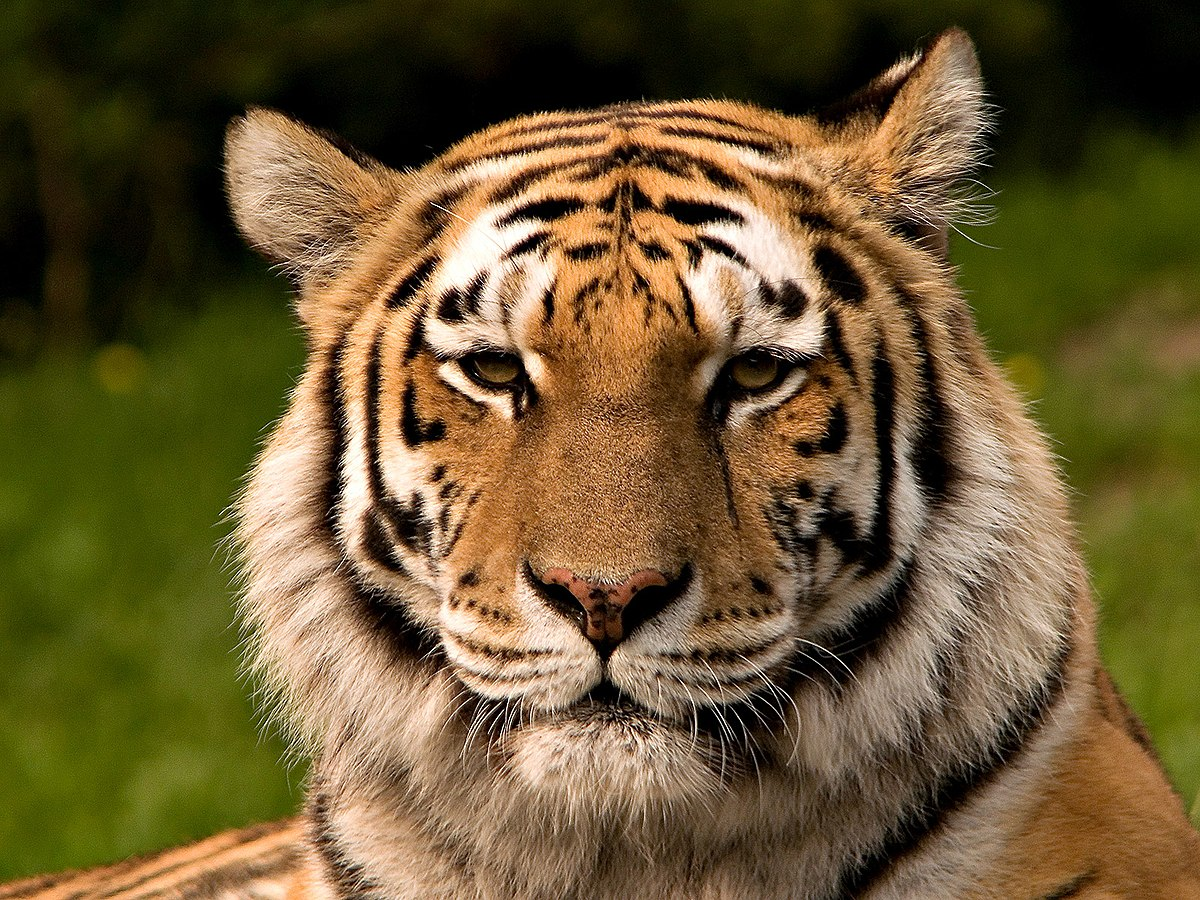
\includegraphics[width = 3cm]{tigre.jpg}
    
    \section*{2. Posicionamiento de im\'agenes}

        \begin{figure}[h!]
            \raggedright
            \subfigure[Imagen a la izquierda]{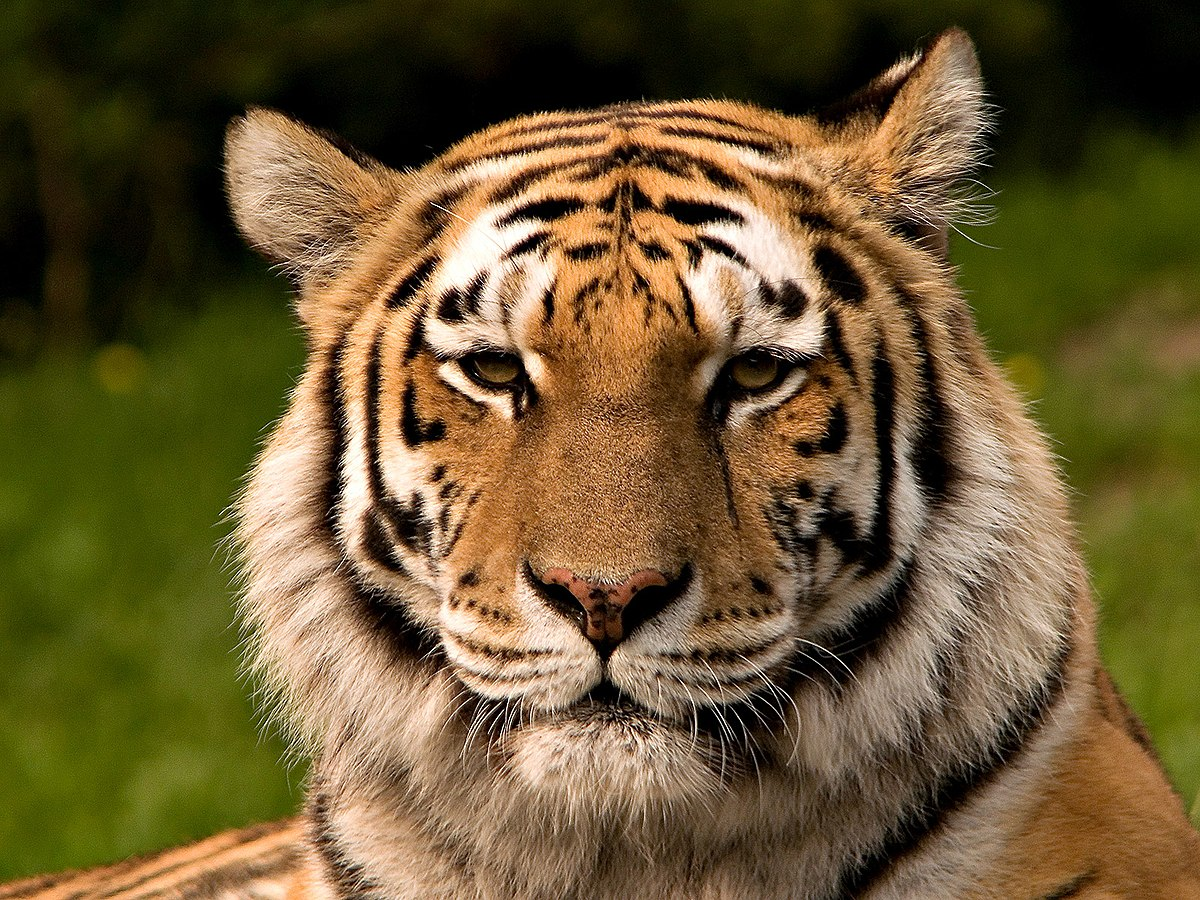
\includegraphics[width = 3cm]{tigre.jpg}}
        \end{figure}
        
        \begin{figure}[h!]
            \centering
            \subfigure[Imagen al centro]{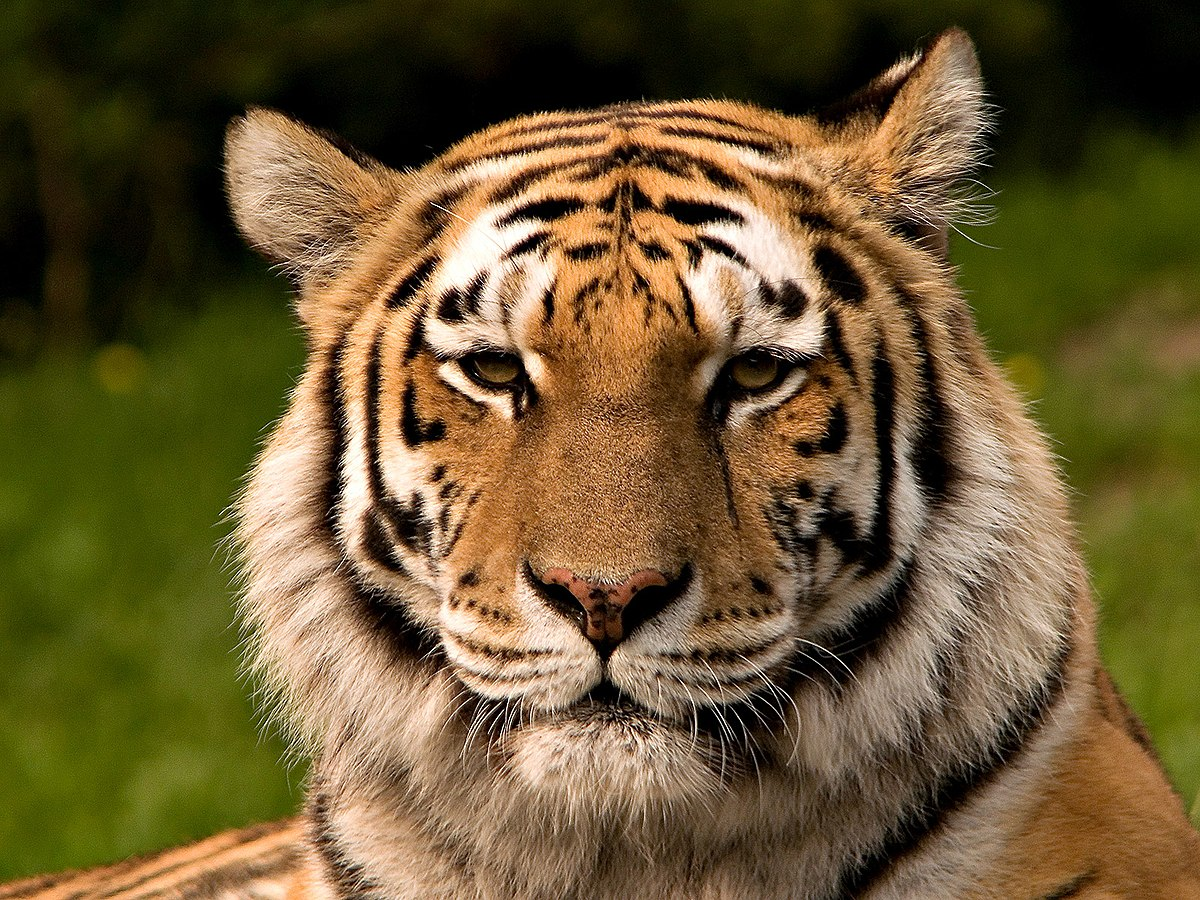
\includegraphics[width = 3cm]{tigre.jpg}}
        \end{figure}

        \begin{figure}[h!]
            \raggedleft
            \subfigure[Imagen a la derecha]{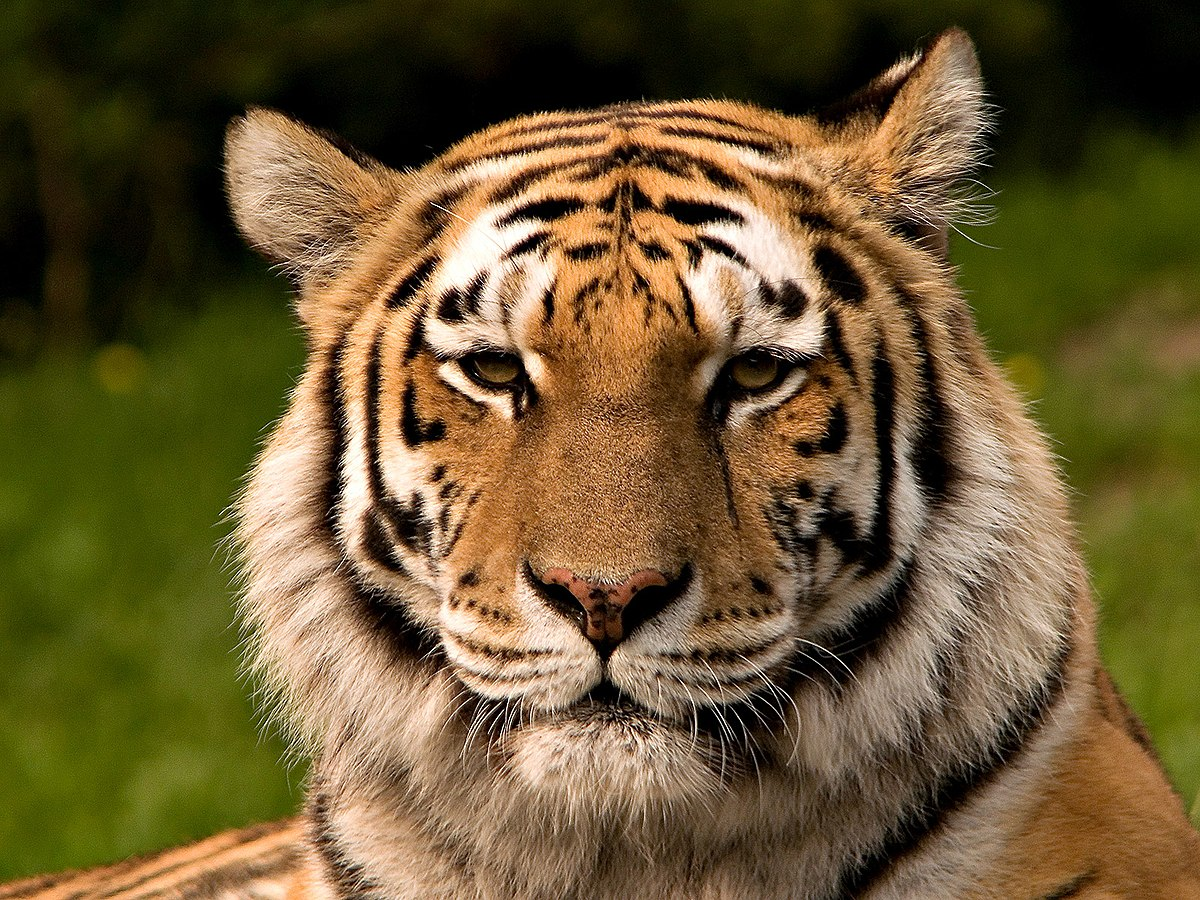
\includegraphics[width = 3cm]{tigre.jpg}}
        \end{figure}

        

    \section*{3. F\'ormulas matem\'aticas}

        \subsection*{3.1 Ecuaciones}
        \subsection*{3.2 S\'imbolos matem\'aticos}
        \subsection*{3.3 Exponenciaci\'on y radicaci\'on}
        \subsection*{3.4 Funciones trigonom\'etricas}

    \section*{4. Inserci\'on de bibliograf\'ia}
\end{document}